\chapter{System Design}

\section{Introduction to System Design}

The SafeSurf system is designed as a machine learning--based real-time phishing detection system that integrates a modern web interface, browser extension, and a scalable backend architecture.
\noindent
The system follows a modular and layered design, consisting of:

\begin{itemize}
    \item React-based frontend and Chrome extension for user interaction
    \item FastAPI backend for request handling and model execution \cite{ref10}
    \item Hybrid ensemble machine learning model for phishing detection \cite{ref11}
\end{itemize}
\noindent
Unlike traditional systems, SafeSurf incorporates:

\begin{itemize}
    \item DNS Guard layer for deterministic early filtering
    \item Asynchronous feature extraction (111 infrastructure and lexical features)
    \item Hybrid ensemble (VotingClassifier + NLP Text model)
\end{itemize}
\noindent
This architecture ensures:

\begin{itemize}
    \item Real-time detection with low latency
    \item High accuracy (exceeding 97\%)
    \item Efficient computational resource utilization
\end{itemize}

\section{System Architecture}

The SafeSurf system is organized into three major layers:

\subsection{Client Layer}

\begin{itemize}
    \item Chrome Extension (real-time background detection)
    \item React Web Dashboard UI (manual URL analysis and metrics)
    \item Displays straightforward verdicts:
    \begin{itemize}
        \item Safe
        \item Phishing Risk
    \end{itemize}
\end{itemize}

\subsection{Processing \& Detection Layer}

\begin{itemize}
    \item FastAPI Backend Engine
    \item URL Canonicalization
    \item Semaphore Concurrency Control
    \item DNS Guard (deterministic NXDOMAIN gate)
    \item Feature Extraction (111 parallel infrastructure features)
    \item Hybrid ML Ensemble Engine (Infrastructure ML + Linguistic NLP)
\end{itemize}

\subsection{Response Layer}

\begin{itemize}
    \item Soft-Voting Merger \& Probability Threshold Engine
    \item Structured JSON Response Builder
    \item Unified Risk Level mapping (HIGH / MEDIUM / LOW)
\end{itemize}

\begin{figure}[H]
\centering
\includegraphics[width=0.82\textwidth]{./images/system-architecture.png}
\caption{System Architecture}
\label{fig:system-arch}
\end{figure}

\begin{figure}[H]
\centering
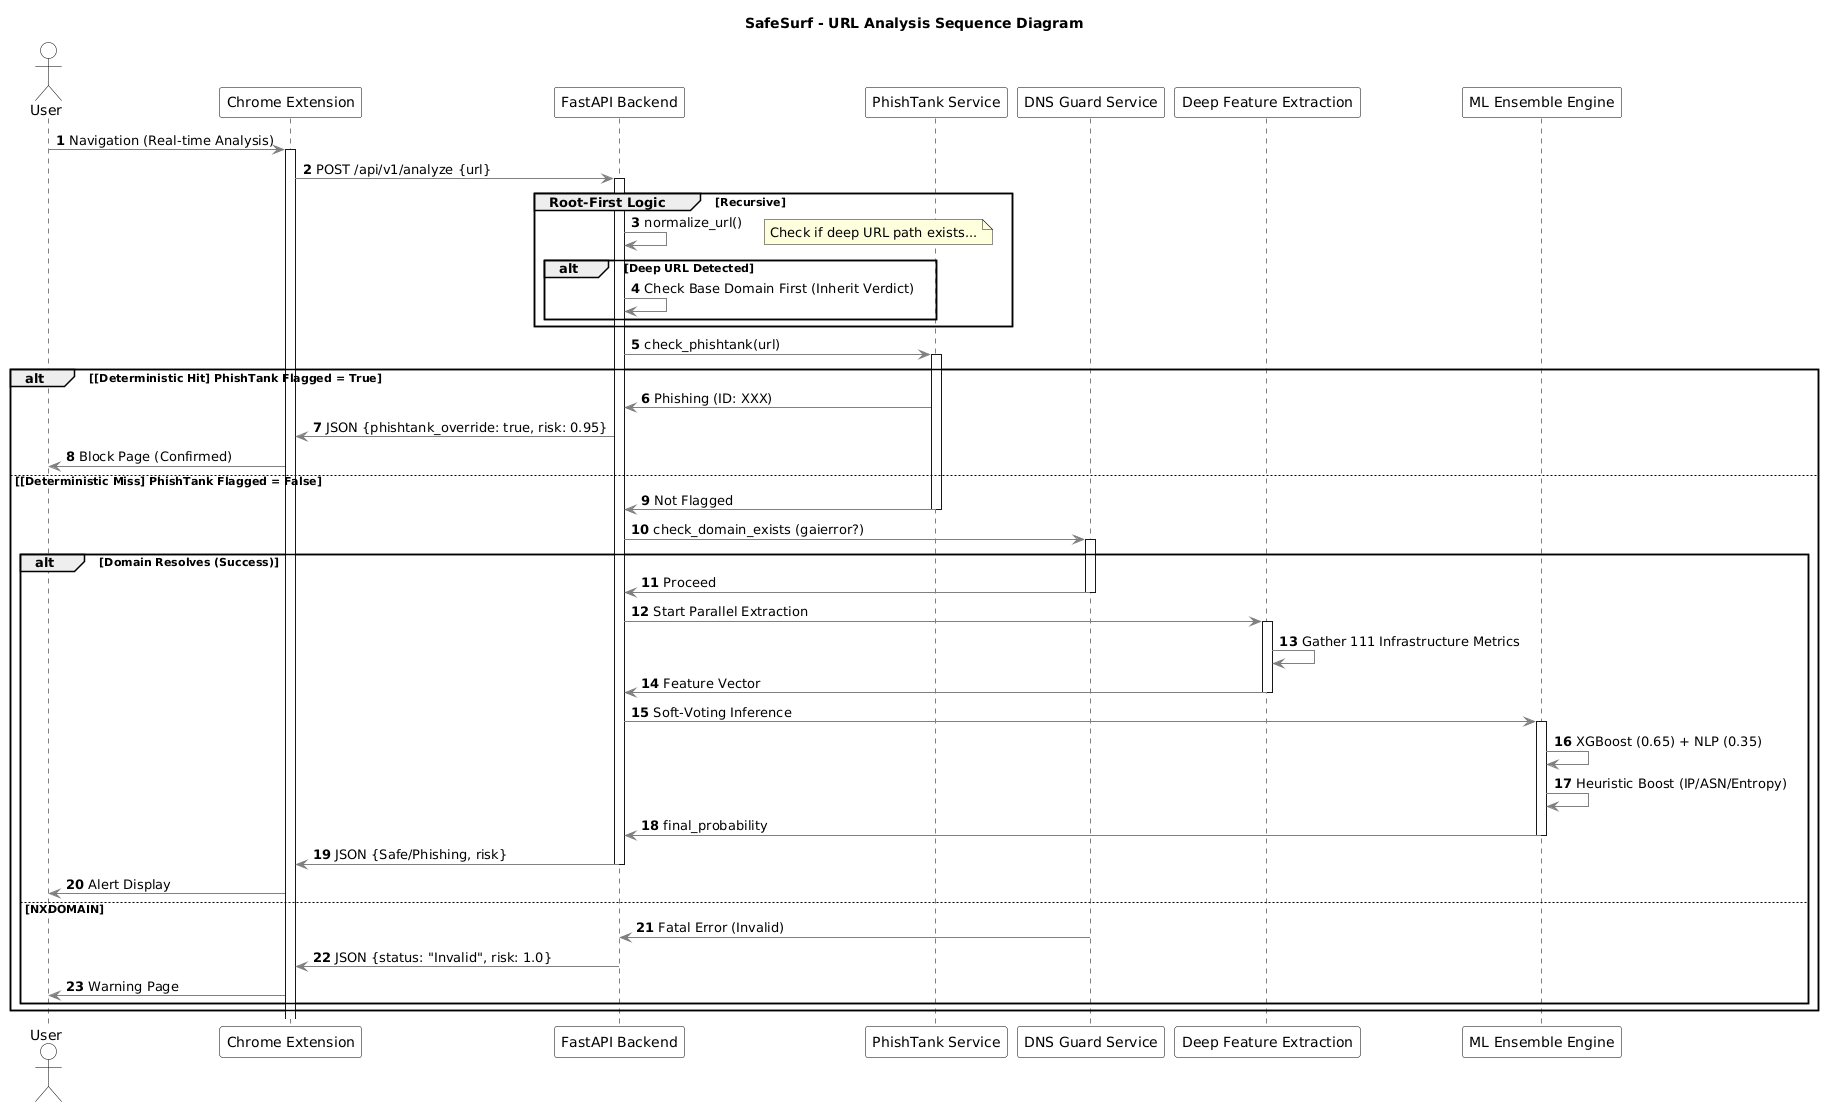
\includegraphics[width=\textwidth]{./images/sequence-diagram.png}
\caption{Sequence Diagram}
\label{fig:sequence_flow}
\end{figure}

\section{System Components}

\subsection{URL Input \& Preprocessing}

\begin{itemize}
    \item Captures URL from:
    \begin{itemize}
        \item Chrome extension passively navigating
        \item Web interface direct manual input
    \end{itemize}
    \item Performs:
    \begin{itemize}
        \item URL normalization (Canonicalization: stripping default ports, collapsing slashes)
        \item Malformed input validation
    \end{itemize}
\end{itemize}

\subsection{DNS Guard Layer}

\begin{itemize}
    \item Acts as the first deterministic security filter
    \item Blocks:
    \begin{itemize}
        \item NXDOMAIN (Non-existent domains)
        \item Dead or unreachable infrastructure
    \end{itemize}
    \item Instantly halts the request, drastically reducing unnecessary ML computation \cite{ref3, ref4}
\end{itemize}

\subsection{Feature Extraction Engine}

\begin{itemize}
    \item Extracts exactly 111 deep features:
    \begin{itemize}
        \item Lexical features (URL structure lengths, character counts, symbol frequencies)
        \item Infrastructure/Network features (WHOIS timing, DNS TTL/Records, SSL certificate validation)
        \item NLP features (Bag-of-Words text token representation)
    \end{itemize}
    \item Leverages:
    \begin{itemize}
        \item Parallel asynchronous processing (\texttt{asyncio.gather})
        \item 15-second strict timeout handling
    \end{itemize}
\end{itemize}

\subsection{Machine Learning Engine}

\begin{itemize}
    \item Specialized Hybrid ensemble system:
    \begin{itemize}
        \item Multi-Model VotingClassifier for Infrastructure (65\% weight)
        \item Logistic Regression NLP model for linguistic text (35\% weight)
    \end{itemize}
    \item Sub-models inside the Voting Ensemble include:
    \begin{itemize}
        \item Logistic Regression
        \item Linear Support Vector Classifier (LinearSVC)
        \item Random Forest Classifier
        \item Histogram-based Gradient Boosting Classifier
        \item Calibrated eXtreme Gradient Boosting (XGBoost) \cite{ref12}
    \end{itemize}
    \item Uses:
    \begin{itemize}
        \item Mathematically weighted soft-voting fusion
    \end{itemize}
\end{itemize}

\subsection{Decision Engine}

\begin{itemize}
    \item Applies exact threshold logic to final probabilities:
    \begin{itemize}
        \item High Risk ($\geq 0.85$ probability)
        \item Medium Risk ($\geq 0.65$ probability)
        \item Low Risk / Safe ($< 0.65$ probability)
    \end{itemize}
\end{itemize}

\subsection{Response Generation}

\begin{itemize}
    \item Maps predictions into a structured JSON response
    \item Sends explicit infrastructure breakdowns and risk verdicts to the UI / Chrome Extension
\end{itemize}

\section{Backend \& Model Implementation}

\subsection{FastAPI Backend}

\begin{itemize}
    \item Handles:
    \begin{itemize}
        \item Scalable API requests optimized natively
        \item Route handling for \texttt{Predict} and \texttt{Metrics}
        \item Complete ML pipeline orchestration
    \end{itemize}
    \item Includes:
    \begin{itemize}
        \item URL canonicalization middlewares
        \item Active concurrency limits (\texttt{Semaphore})
        \item \texttt{MAX\_REQUEST\_BODY\_BYTES} rejection limiters
    \end{itemize}
\end{itemize}

\subsection{Hybrid Ensemble Model}

\begin{itemize}
    \item Combines independent ML probability sequences
    \item Improves:
    \begin{itemize}
        \item Decision accuracy by blending lexical text limits with deep infrastructure realities
        \item Generalization without overfitting
    \end{itemize}
    \item Uses:
    \begin{itemize}
        \item Incremental phase training checkpoints
        \item A Weighted Soft-Voting algorithm fusing the distinct models
    \end{itemize}
\end{itemize}

\section{Frontend \& UI Design}

\begin{itemize}
    \item Developed using React.js \cite{ref9}
    \item Provides:
    \begin{itemize}
        \item A simple, isolated URL input interface
        \item Clear, abstracted result displays hiding raw statistical complexity
    \end{itemize}
    \item Chrome extension:
    \begin{itemize}
        \item Safely captures active tab URLs
        \item Unintrusively displays real-time warnings upon threshold breach
    \end{itemize}
\end{itemize}

\section{Model Design \& Optimization}

\subsection{Feature Engineering}

\begin{itemize}
    \item Isolates distinct analytical paths:
    \begin{itemize}
        \item URL-based lexical feature extraction
        \item Deep Network/Infrastructure querying
        \item NLP Tokenization (CountVectorizer)
    \end{itemize}
\end{itemize}

\subsection{Hybrid Ensemble Model Fusion}

\begin{itemize}
    \item The Scikit-learn VotingClassifier interprets exclusively structured integer/float matrices
    \item The independent NLP Logistic model assesses textual patterns alone
    \item Combined directly at the application service layer via a hard-coded Weighted Soft-voting mechanism
\end{itemize}

\begin{figure}[H]
\centering
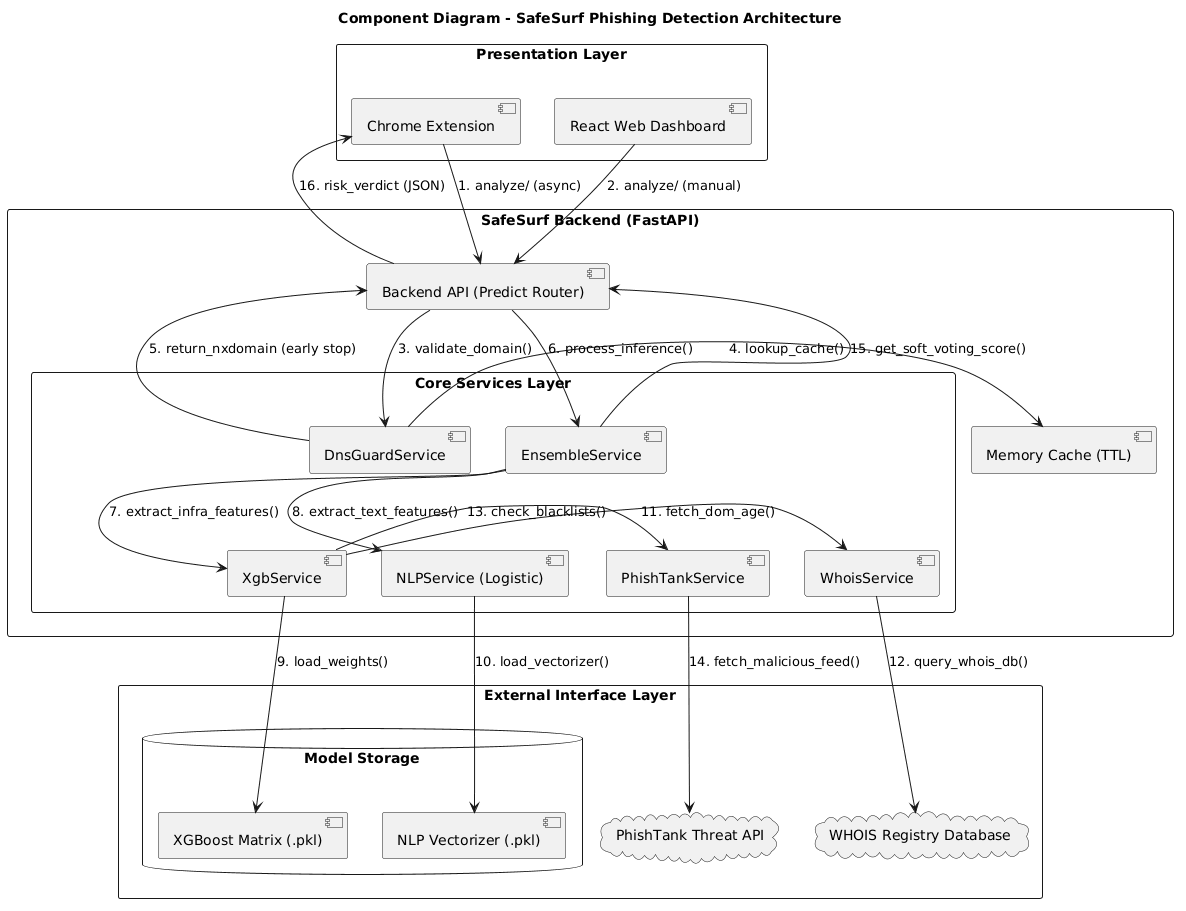
\includegraphics[width=0.85\textwidth]{./images/component-diagram.png}
\caption{System Component Architecture}
\label{fig:component_architecture}
\end{figure}

\section{Development Workflow}

\begin{figure}[H]
\centering
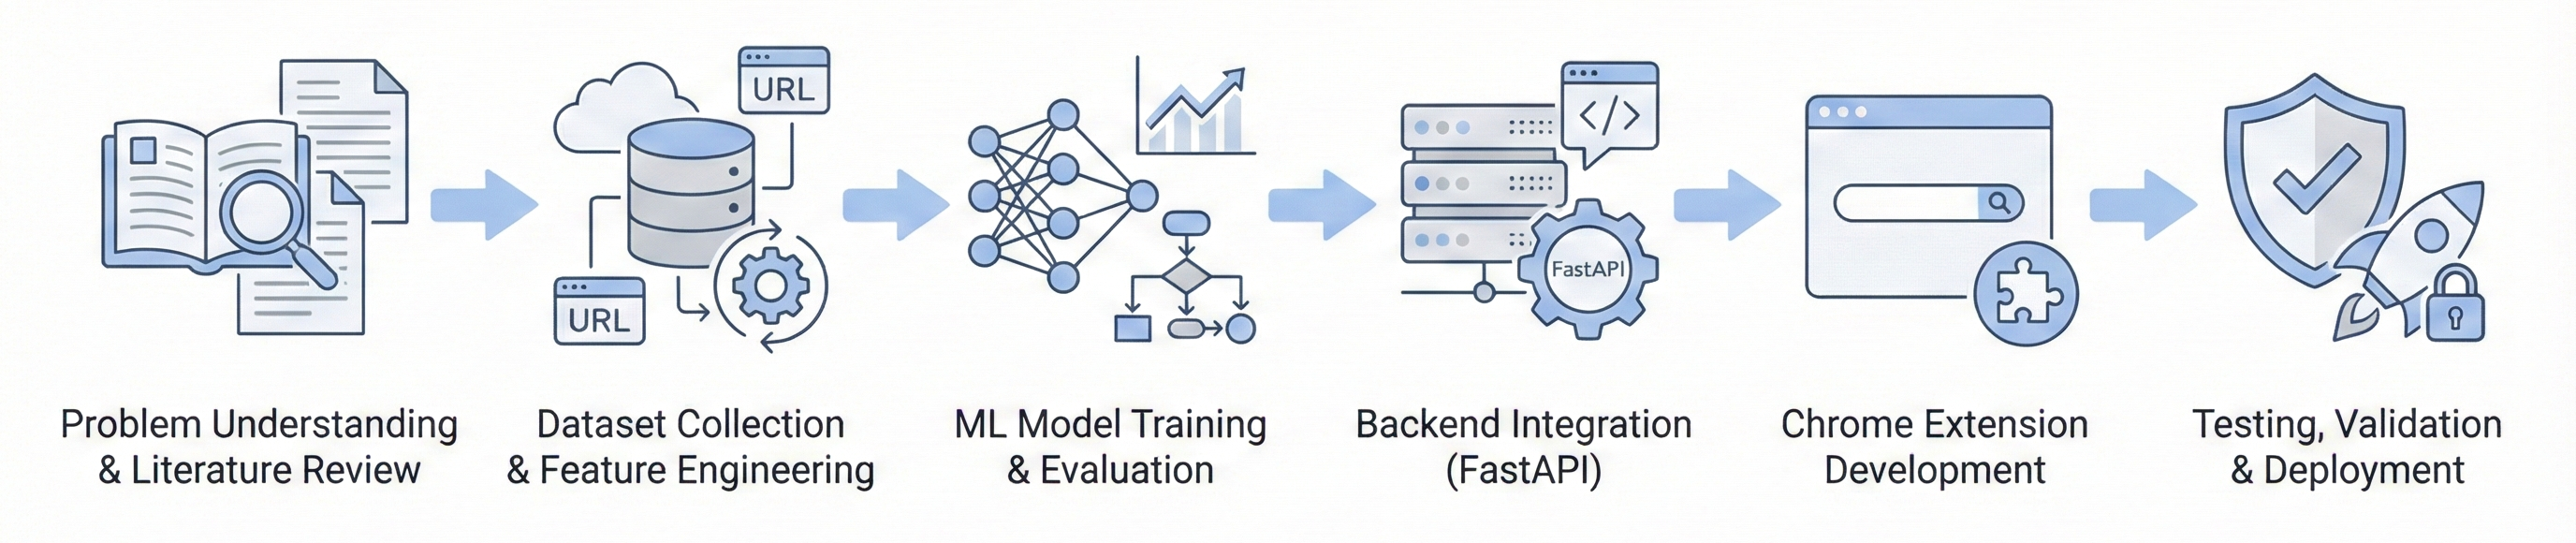
\includegraphics[width=0.9\textwidth]{./images/developmemt-workflow.png}
\caption{Workflow}
\label{fig:workflow}
\end{figure}

\subsection*{Workflow Steps:}

\begin{enumerate}
    \item Problem Understanding \& Structural Architecture Design
    \item Phase 1: Massive Feature Dataset Extraction (PhiUSIIL Database \cite{ref5})
    \item Phase 2: Feature Engineering \& Tokenization
    \item Phase 3: Model Training \& Sanity Validation Iterations
    \item Backend Integration (FastAPI Soft-Voting orchestrator)
    \item Chrome Extension \& React Web Application Development
    \item Testing, Hot-Reload Testing, \& Final Deployment
\end{enumerate}

\section{Conclusion}
\noindent
The SafeSurf system design formally asserts a scalable, highly efficient, and intelligent architecture for modern phishing detection.
\noindent
By integrating:

\begin{itemize}
    \item Deterministic DNS-based filtering
    \item Hybrid machine learning ensemble fusions
    \item Real-time concurrent API processing
\end{itemize}
\noindent
the system reliably ensures:

\begin{itemize}
    \item Accurate detection ($\geq 97\%$)
    \item Fast programmatic response profiles ($\leq 500$ ms)
    \item User-friendly, frictionless interactions
\end{itemize}
\noindent
Future enhancements such as continuous data-drift telemetry alerting and cloud container orchestration \cite{ref14} will further fortify system performance and global scalability.
